\chapter{Software Architecture Design}
\label{chap:software-architecture-design}
<TIP: Describe how you design your application using Unified Modelling
Language (UML). There should be at least two diagrams that describe the
software architecture. You may add additional or remove unnecessary diagrams.
However, there needs to be a coherency between them at the end./>

\section{Domain Model}
\label{section:domain-model}
<TIP: Describe the business concept of your project. Showcase a
domain model that captures the said concept./>

\section{Design Class Diagram}
\label{section:design-class-diagram}
<TIP: Showcase a design class diagram for your project and explain
how it works here. You can group classes into packages or layers to communicate your
design better./>

\section{Sequence Diagram}
\label{section:sequence-diagram}
<TIP: Sequence diagrams describe how the software runs at runtime.
You do not have to create a sequence diagram for every scenario. However,
there should be one for all the main ones./>

<ChatGPT: Creating a sequence diagram for every use case is not
strictly necessary, but it can be a valuable tool in certain situations. Sequence
diagrams are particularly useful for illustrating the interactions between different
components or objects in a system over time, showcasing the flow of messages
or actions between them./>

\section{Algorithm}
\label{section:algorithm}
<TIP: Optional, If you are working on a research project that proposes a new
algorithm, you can describe your algorithm here. It can be in the form of
pseudocode or any diagram that you deem appropriate./>

\section{AI Component}
\label{section:ai-component}

\subsection{Model Selection}
\label{subsection:model-selection}

For this project, \textbf{OpenThaiGPT-14B} has been selected as the base AI model. This decision is based on its strong proficiency in the Thai language, 
making it well-suited for the analysis of Thai stock market documents and investment assistance tailored to Thai investors\cite{yuenyong2024openthaigpt15thaicentricopen}.

\begin{figure}[h]
    \centering
    \frame{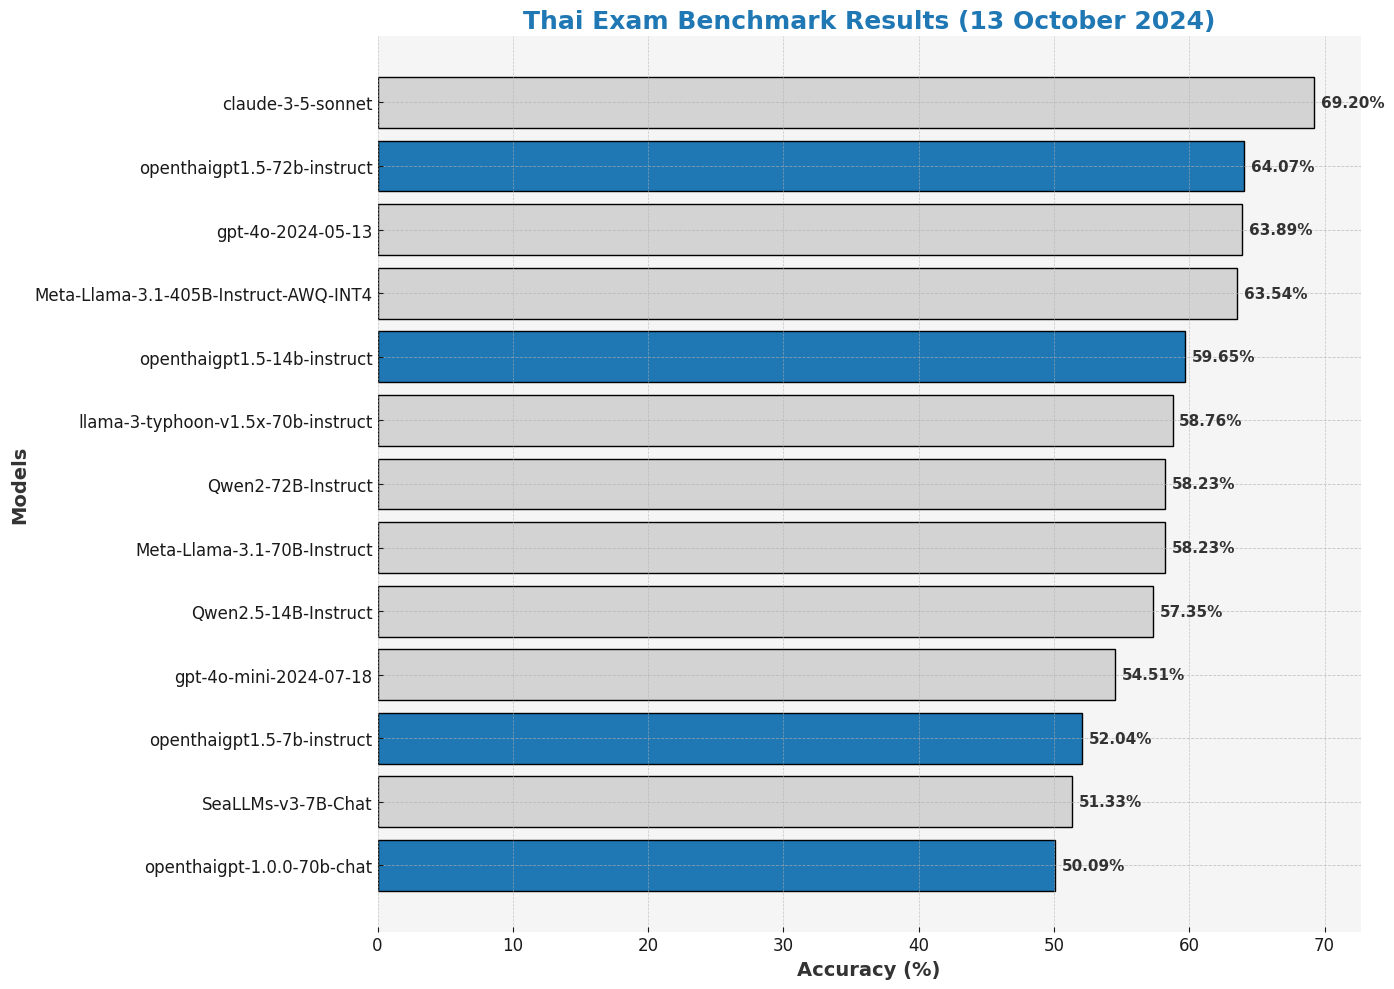
\includegraphics[width=0.6\textwidth]{chapter-4/openthaigpt-thai-exam-benchmark.png}}
    \caption[Performance of OpenThaiGPT on Thai Exam Benchmark]{Benchmark performance of OpenThaiGPT compared to other large language models on the Thai Exam (13 October 2024), accessed 20 March 2025, \url{https://openthaigpt.aieat.or.th/}.}
    \label{fig:openthaigpt-thai-exam-benchmark}
\end{figure}

\FloatBarrier

OpenThaiGPT has demonstrated competitive performance against leading models in Thai language processing.
Figure \ref{fig:openthaigpt-thai-exam-benchmark} presents benchmark results comparing OpenThaiGPT with other AI models on a standardized Thai language exam.
OpenThaiGPT-1.5-72B-Instruct achieved 64.07\% accuracy, surpassing GPT-4o-2024-05-13 and other large-scale models such as Meta-Llama-3.1-405B-Instruct-AWQ-INT4. 
Furthermore, OpenThaiGPT-1.5-14B-Instruct achieved 59.65\% accuracy, demonstrating strong performance even with a smaller model configuration\cite{OpenThaiGPT}.

\begin{itemize}[leftmargin=60pt]
    \item \textbf{Thai Language Proficiency}: It performs on par with larger models in Thai language understanding and generation.
    \item \textbf{Optimized for Thai NLP Tasks}: OpenThaiGPT is trained on extensive Thai-language corpora, making it highly capable in understanding and generating Thai text. This linguistic strength provides a solid foundation for further fine-tuning on stock market–specific tasks.
    \item \textbf{Scalability and Efficiency}: The 7B, 14B, and 72B parameter versions allow us to select the best balance between computational cost and performance based on deployment needs.
\end{itemize}

\subsection{Training Data}
\label{subsection:training-data}

The model will be fine-tuned using a curated dataset comprising publicly available Thai financial data. 
Both structured and unstructured data sources will be included to ensure the model has a comprehensive understanding of the Thai stock market, investment principles, and stock analysis techniques.

\begin{itemize}[leftmargin=60pt]
    \item \textbf{56-1 One Reports}: Annual reports of publicly listed Thai companies, published by the Securities and Exchange Commission (SEC) of Thailand. These reports contain essential information, including financial statements, business strategies, and management discussions.
    \item \textbf{Financial Statements}: Standardized financial documents, including balance sheets, income statements, and cash flow statements, sourced from companies listed on the Stock Exchange of Thailand (SET). These help the model learn how to interpret financial health and performance indicators.
    \item \textbf{Thai Stock Investment Literature}: Books and educational materials focused on investing in the Thai stock market, covering strategies, technical and fundamental analysis tailored to Thai stocks, and locally relevant valuation models. These resources help the model produce insights aligned with theories and practices recognized by Thai investors.
    \item \textbf{Synthetic Thai Stock Q\&A Dataset}: A custom-generated dataset comprising questions and responses related to Thai stocks. This synthetic data is intended to improve the model’s performance on domain-specific question answering tasks.
\end{itemize}

\subsection{Model Fine-Tuning}
\label{subsection:model-fine-tuning}

To adapt OpenThaiGPT to the domain of Thai stock investment, supervised fine-tuning will be conducted using the curated dataset described in Section~\ref{subsection:training-data}. 
The goal of this process is to align the model’s output with domain-specific language, terminology, and reasoning relevant to the Thai stock market.

\begin{itemize}[leftmargin=60pt]
    \item \textbf{Dataset Formatting}: Training samples will follow an instruction-based format, consisting of a clearly defined task prompt, optional contextual input, and the corresponding target output (e.g., an analysis of a selected stock or a summary of current price trends).
    \item \textbf{Fine-Tuning Methodology}: Fine-tuning will utilize Quantized Low-Rank Adaptation (QLoRA), a parameter-efficient method that introduces trainable components into select layers of the pre-trained model while keeping the majority of weights frozen. This method significantly reduces computational requirements and is well-suited for environments with limited hardware resources\cite{QLoRAMedium2023}.
\end{itemize}

\subsection{Evaluation and Metrics}
\label{subsection:evaluation-and-metrics}

The performance of the fine-tuned OpenThaiGPT model will be evaluated using a combination of automated and expert-driven evaluation methods. 
These methods are designed to assess the model's effectiveness across three key dimensions: understanding, quality, and correctness.

\begin{itemize}[leftmargin=60pt]
    \item \textbf{Semantic Similarity (Understanding)}: This metric will evaluate how well the model captures the intended meaning of a query. Sentence embeddings will be used to compute cosine similarity between the model’s output and a reference answer, ensuring semantic alignment even when the phrasing differs\cite{SemScore2024}.
    \item \textbf{GEval (Quality)}: GEval is a generative evaluation tool that assesses the overall quality of generated text based on relevance, coherence, and completeness. This is particularly suitable for evaluating tasks such as financial summaries and analytical explanations\cite{GEval2024}.
    \item \textbf{Pass Rate (Correctness)}: The pass rate will measure the proportion of responses that meet predefined correctness criteria. This is especially useful for fact-based or calculation-driven tasks where an objectively correct answer is expected.
    \item \textbf{User Satisfaction (Expert Feedback)}: In addition to automated evaluations, qualitative feedback will be collected through a structured survey conducted with Thai financial experts. Experts will assess a representative sample of model outputs based on clarity, usefulness, and accuracy. Their insights will provide valuable input on the model's practical effectiveness and trustworthiness in real-world scenarios.
\end{itemize}

The combination of these evaluation strategies will ensure a comprehensive understanding of the model’s capabilities and limitations in supporting Thai investors with reliable, high-quality, and context-aware responses.
